\chapter{Planificación}
\label{chapter:planificacion}

\section{Riesgos}
\subsection{Identificación y análisis}
%% Identificación y analisis
%Además de los típicos (inundaciones o incendios) hay otros relacionados con la seguridad informática, protección de datos, o con otros aspectos más empresariales.

Con la estructura que hemos definido anteriormente descartamos una gran cantidad de riesgos comunes a infraestructuras similares. Un ejemplo puede ser el acceso físico no autorizado a los servidores, el fallo hardware o desastres naturales. Los servicios en la nube de Google nos proporcionan sus capas de seguridad físicas\cite{GCPSecurity}.

A continuación vamos a definir alguno de los riesgos más probables para nuestra tipología de red y metodología de trabajo.
\begin{itemize}
    % \item \textbf{Virus informáticos:} Son los riesgos más comunes y peligrosos en cuanto a software. Una  con nuestras características debe blindarse para evitar la entrada de virus y ciberdelincuentes, además de disponer de un plan de protección y recuperación.
    \item \textbf{Accesos no autorizados:} La imposibilidad de disponer de los recursos empresariales únicamente en la red local nos obliga a exponer una puerta de entrada de forma global. Para evitar la entrada de individuos no deseados se deben aplicar filtros. Estos filtros no solo deben aplicar a quienes tienen permitido el acceso general, sino que puede ver y editar cada usuario de forma individual según su cargo de responsabilidad en la empresa. Este tipo de sucesos pueden ser poco frecuentes, pero fácilmente detectables y sus consecuencias pueden minimizarse.%La posibilidad de teletrabajo implica que el acceso no puede restringirse a direcciones IP determinadas mediante una whitelist.
    \item \textbf{Filtración de datos:} Exponer los datos en Internet puede causar una filtración de información que podría ser intencionada o no. Este es el riesgo más probable y difícil de identificar, lo puede ocasionar un empleado con acceso lícito. Para paliar esto se puede usar un sistema de monitoreo de red.
    \item \textbf{Denegación de servicio:} Al tener los servidores expuestos a Internet, existe la posibilidad de sufrir ataques que los saturen e impidan el acceso a los recursos internos.
    \item \textbf{Ransomware:} Los ciberdelincuentes estarán constantemente atacando nuestros servidores en busca de vulnerabilidades para robar y cifrar la información y poder pedir un rescate. Se deben bastionar los servidores y disponer de un plan de acción para evitar estos sucesos. Este tipo de suceso es poco probable que ocurra, pero, de hacerlo, tendría graves consecuencias.
\end{itemize}
\subsection{Plan de acción}
%% Plan de acción
%Basado en lo descrito en el punto anterior, indicar qué importancia tiene, la probabilidad de que pase,  y las medidas a tomar para evitarlo o minimizarlo.
\subsubsection{Medidas físicas}
Tal y como hemos comentado en el punto anterior, los servidores estarán alojados en los centros de datos de Google. Todos los CPD de esta empresa son de su propiedad y no alquilan estos servidores a otros proveedores\cite{GCPSecurity}. Cuentan con políticas de duplicado de información en centros de respaldo y construcción de estos lejos de zonas propensas a inundaciones, terremotos o huracanes. En cada centro disponen de sistemas de detección infrarrojos y láser, control de acceso biométrico, barreras contra vehículos y más\cite{GoogleWhitepaper}.

% \begin{center}
% \noindent\rule{5cm}{0.5pt}
% \end{center}

Google dispone de alguna normativa de seguridad en cuando a software, como puede ser la firma criptográfica de sus servicios internos para evitar suplantaciones o un sistema de arranque y BIOS segurizados a bajo nivel.

\subsubsection{Protección DNS}

Para evitar los ataques de denegación de servicio contrataremos los servicios de Cloudflare. Esta empresa se dedica exclusivamente a fortificar y mejorar las comunicaciones entre el exterior y los servidores expuestos mediante NaaS\footnote{\textit{Network as a Service} o Red como Servicio.}. Para ello se nutre de distintas herramientas como proxies DNS, servidores caché y túneles seguros. En este proyecto aprovecharemos la gestión DNS disponible en la versión gratuita.

Los proxies DNS de Cloudflare nos permiten enmascarar nuestras IP públicas y registros DNS. Cualquier consulta DNS que realice un cliente hacia nuestro dominio obtendrá un único registro DNS. Además, el sistema de detección de Cloudflare hará que los ataques DoS ni siquiera llegue a nuestra infraestructura\footnote{Cuando un visitante accede por primera vez a una página, Cloudflare  obliga a su navegador a pasar por un reto de JavaScript y le otorga una cookie identificatoria. Este proceso es transparente para el usuario. Si se realizan muchas peticiones desde una misma IP o desde un mismo equipo, solicitará al usuario resolver un Captcha. En algunos casos bloqueará el acceso. Si el acceso lo realiza una máquina sin intervención de un usuario, el reto JavaScript no podrá ser completado.}.

Las peticiones de los clientes también vendrán directamente del proxy, por lo que se pueden crear filtros para denegar todo acceso que intente saltarse los bloqueos de Cloudflare.

\begin{figure}[H]
  \centering
  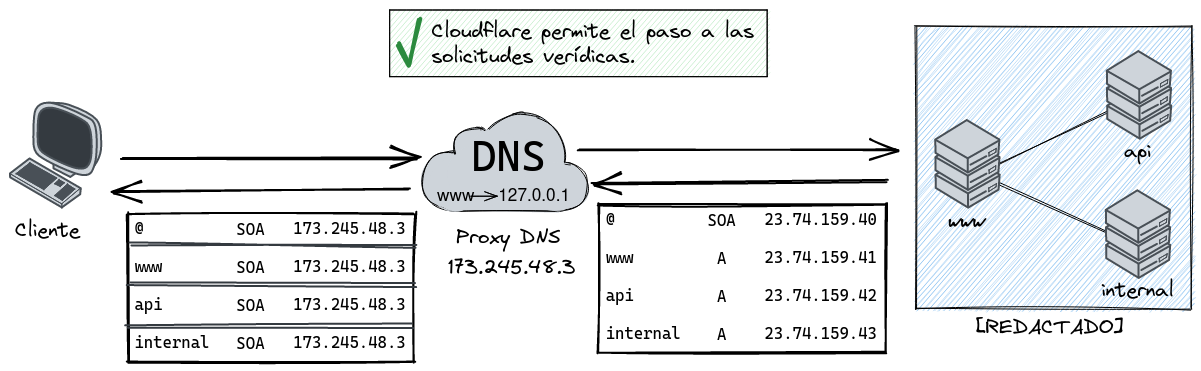
\includegraphics[width=0.7\textwidth]{figura2.png}
  \caption{Petición legítima aceptada}
  \label{fig:DNSProxyAceptado}
\end{figure}
\begin{figure}[H]
  \centering
  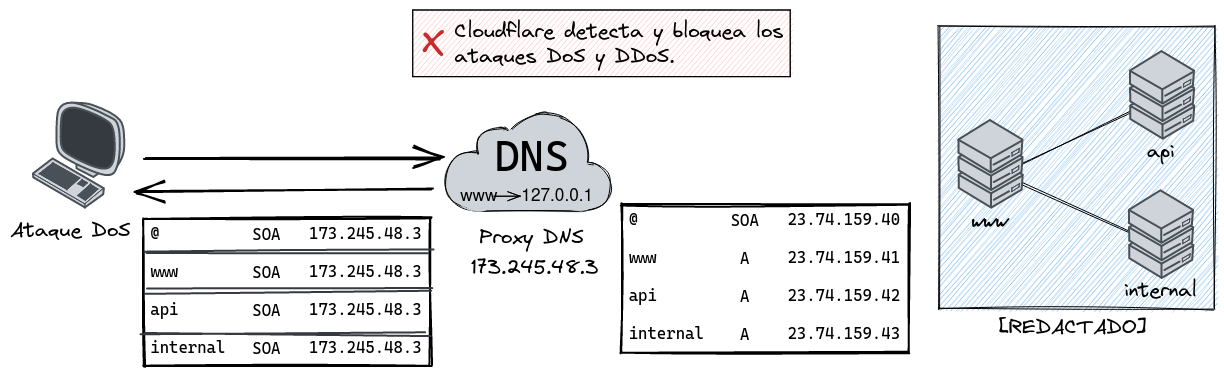
\includegraphics[width=0.7\textwidth]{figura3.png}
  \caption{Ataque rechazado}
  \label{fig:DNSProxyRechazado}
\end{figure}

Como se puede apreciar en las figuras \ref{fig:DNSProxyAceptado} y \ref{fig:DNSProxyRechazado}, los registros DNS de Cloudflare no solo ocultan nuestras direcciones reales, sino que aísla los registros para evitar descubrir mediante escaneos la cantidad de subdominios presentes.

\subsubsection{Seguridad activa}

Monitorizar la actividad de nuestra red interna es esencial para detectar intrusos y actividades anómalas. Existe una gran cantidad de herramientas pensadas para estos. Las pilas de monitorización son conjuntos de software trabajando al unísono que se dedican a recopilar, agrupar e interpretar los registros y estados de distintos sistemas. Estos entornos, siendo Node\_exporter (recopilación), Prometheus (agrupación) y Grafana (interpretación) el más conocido, son extremadamente potentes y altamente configurables, pero el tiempo requerido para su implementación nos obliga a descartarlo para este proyecto.

En su lugar, una solución privativa de un producto tipo EDR\footnote{De las siglas en inglés "\textit{Endpoint Detection \& Response}", es un software dedicado a la detección, eliminación y monitorización de brechas de seguridad. También permite la detección y seguimiento de ataques informáticos a tiempo real. Los EDR se consideran los antivirus de nueva generación.} que nos permitirá controlar la salud de los servidores y vigilar las posibles brechas de seguridad. Al ser un producto empresarial especializado es complicado obtener licencias de prueba, por lo que este producto no se implementará en el proyecto.

\subsubsection{Seguridad pasiva y política de copias de seguridad}

En caso de ataque exitoso se tomarán los planes de acción que ya tenía predefinidos la empresa por su departamento de sistemas. Este proyecto contempla la modularidad de las conexiones y facilita el aislamiento del o los equipos infectados del resto de la red. En caso de que un cliente se encuentre infectado, el ciberdelincuente no podrá realizar movimientos laterales dentro de la red, la VPN se configurará de forma que todos los equipos estarán aislados entre ellos.

Una de las ventajas que se tienen al usar sistemas virtualizados en la nube es que podemos realizar instantáneas de las máquinas sin necesidad de pararlas. Estas se almacenan dentro de los centros de datos de Google. 

\subsubsection{Autenticación y autorización}

La autenticación se realizará mediante par de claves y contraseña usando la conexión por la VPN tal y como se indica en el anexo \ref{anexo:a}. Los servicios

% RECURSOS
% HUMANOS, MATERIALES Y PRESUPUESTO
\section{Recursos}
\subsection{Humanos}
La implementación de la red, gran parte del proyecto, la realizará Nicolás como único integrante del proyecto. Del resto de las funciones se encargará el departamento de sistemas de la empresa. Para aquellas implementaciones de software que se necesite, también la realizará [REDACTADO] simulando a otro empleado.
\subsection{Materiales}
A continuación listamos los recursos que utilizaremos:
\begin{itemize}
    \item \textbf{Google:} Recursos que utilizaremos dentro del entorno de Google Cloud Platform:
    \begin{itemize}
        \item \textbf{Servidor interno:} Usaremos el servidor N1 micro de Google, es el que dispone de los recursos más bajos (un procesador virtual y 614 MB de memoria RAM). Usará Debian Stable y tendrá un contenedor Docker con Nextcloud y una base de datos.
        \item \textbf{Servidor de acceso:} Una máquina N1 micro con el servidor OpenVPN
        \item \textbf{Servidor API:} La creación y mantenimiento del contenido será responsabilidad de los departamentos de desarrollo. Para las pruebas de acceso solo instalaremos el servidor SSH.
        \item \textbf{Bucket de copias de seguridad:} Volumen lógico en la nube tipo Nearline\footnote{Google cobra por el acceso a los datos de los buckets. Tiene distintos niveles según las veces que se quiera acceder para descargar los datos. Nearline es un nivel intermedio donde el GB cuesta 0,01 USD al mes si se consulta una vez al mes como máximo. Es el recomendado para copias de seguridad.} de tamaño variable.
    \end{itemize}
    \item \textbf{Cloudflare:} Aunque se use la cuenta gratuita, se usarán el registro DNS y el proxy DNS de Cloudflare.
    \item \textbf{Cliente Linux:} Para el acceso global a la infraestructura y la documentación, usaré mi equipo personal con Manjaro GNOME 42.
    \item \textbf{Cliente Windows:} Simulando un equipo del departamento de Diseño gráfico, usaré un cliente Windows 11 virtualizado.
    \item \textbf{Cliente Linux virtualizado:} Para la conexión simulando equipos de otros departamentos se usará un sistema Ubuntu 22.04 LTS virtualizado.
\end{itemize}
\subsection{Presupuesto}

A falta de una factura proforma, se va a realizar un presupuesto aproximado usando los datos estimados de las consolas de los servicios. En el caso de Cloudflare, se usará la cuenta gratuita. Las condiciones de uso de Cloudflare no limitan este plan al uso personal, por lo que podrá ser usado en un entorno empresarial real si es suficiente\cite{CloudflareTerms}. Los buckets de Google no tienen un tamaño fijo, van aumentando solos a medida que se llena el espacio. Para este presupuesto vamos a simular 10 GB de información.

\begin{table}[h!]
\centering
\begin{tabularx}{\textwidth}{|r|X|c|c|c|}
\hline
Plataforma     & Producto       & Precio unitario & Cantidad & Total             \\ \hline
Google         & N1 Micro       & 5,39 USD        &    3     & 16,17 USD         \\
               & Bucket Nearline& 0,01 USD/GB     & 1\times10 GB  & 0,1 USD      \\
               & Instantáneas   & 0,019 USD/GB    & Calcular & X USD             \\ \hline
Cloudflare     & Cuenta gratuita& 0 USD           & 1        & 0 USD             \\ \hline
Nextcloud      & Nextcloud Hub  & 0 USD           & 1        & 0 USD             \\ \hline
Siteground     & Dominio        & 1,08 USD        & 1        & 1,08 USD          \\ \hline
Microsoft      & Windows 11 Enterprise Evaluation & 0 USD & 1 & 0 USD            \\ \hline
Sumatorio      &                &                 &          & 17,35 USD/mes     \\ \hline \hline
Personal       & Técnico        & 35 €/h           & 9 horas  & 315 €            \\ \hline
\end{tabularx}
\label{tab:presupuesto}
\end{table}

\section{Tareas, definición y temporización}
%% TAREAS, DEFINICIÓN Y TEMPORALIZACIÓN
% Definición de tareas
Simulando que la empresa se encuentra en proceso de adaptación, dividiremos las tareas en cuatro etapas: Creación, comprobación, solución de errores y migración. Las tareas se ejecutarán de una en una y se comprobará su correcto funcionamiento de forma individual y mitigarán los posibles errores que aparezcan. Cuando se hayan completado todas, podremos realizar una comprobación global. Cuando se resuelvan los errores que aparecieron en la anterior fase y consideremos la infraestructura como estable, comenzaremos a migrar los distintos departamentos a la nueva infraestructura, así su trabajo no se verá interrumpido.
% Asignación de recursos a las tareas
% Temporalización de las tareas
% Diagrama de GRANTT
\section{Diagrama de Gantt}
A continuación se muestra el diagrama con la planificación del periodo de ejecución.

\begin{figure}[H]
  \centering
  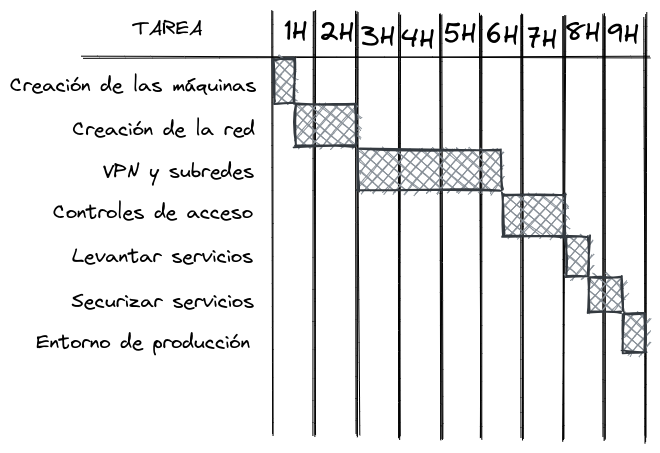
\includegraphics[width=0.7\textwidth]{gantt.png}
  \label{fig:gantt}
\end{figure}
%DEFINICIÓN DEL SEGUIMIENTO
%
% Definir cómo se va a controlar la ejecución del proyecto. No se trata de hacer el seguimiento, sino establecer cómo se va a realizar
% Valoración de la consecución de la tarea
% Calcular la desviación de tiempo empleado frente al planificado
% Calcular la desviación de presupuesto empleado frente al planificado
% Calcular la desviación de recursos empleados frente al planificado

\section{Definición del seguimiento}

Para el seguimiento utilizaremos SuperProductivity, un programa de software libre para la planificación y seguimiento de tareas. Indicaremos en cada tarea las distintas fases y el tiempo planificado y el dedicado para cada tarea. 

\begin{figure}[H]
  \centering
  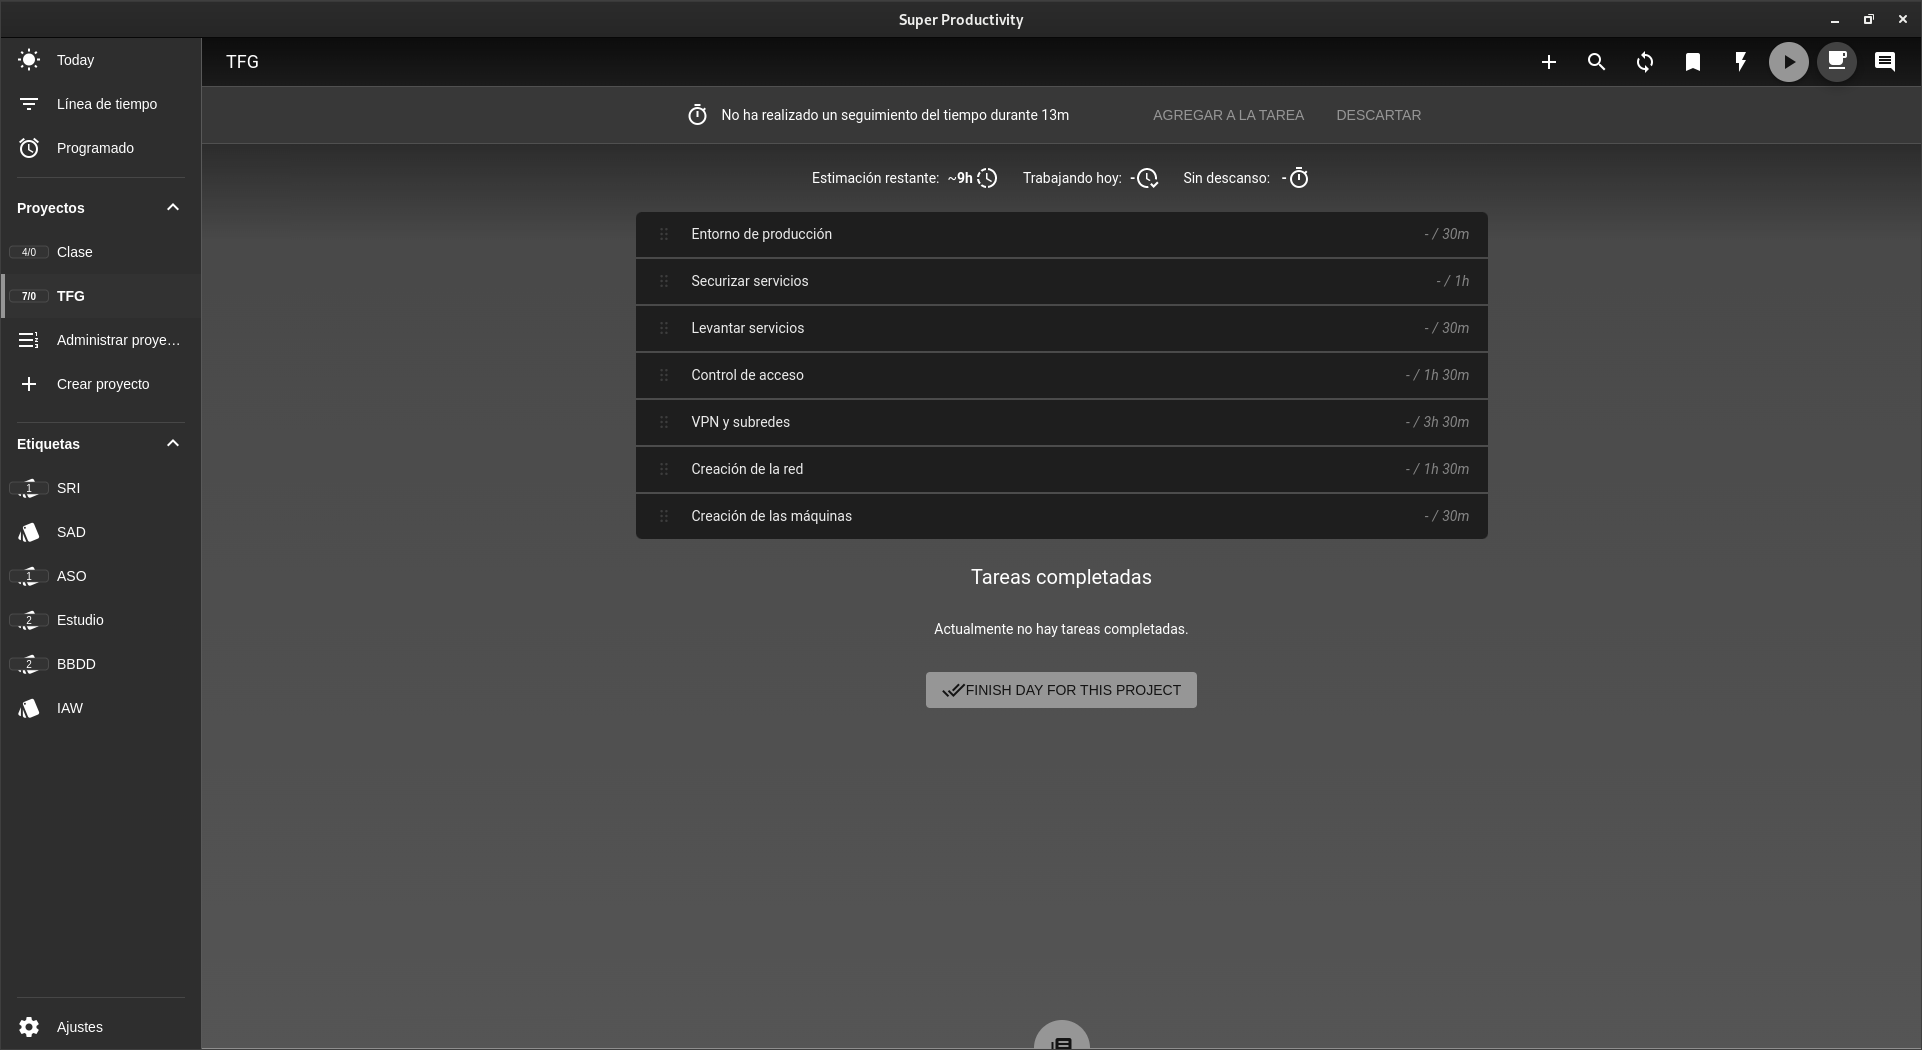
\includegraphics[width=0.7\textwidth]{figura5.png}
  \label{fig:superproductivity}
  \caption{SuperProductivity con las tareas y tiempo definido.}
\end{figure}

Además, usaremos la siguiente tabla para plasmar la información.
\begin{table}[h!]
    \centering
\begin{tabularx}{\textwidth}{|>{\centering\arraybackslash}X|>{\centering\arraybackslash}X|}
\hline
\multicolumn{2}{|>{\columncolor[gray]{.8}}c|}{Tarea} \\ \hline
\multicolumn{2}{|c|}{  } \\ \hline
\rowcolor[gray]{.8} Tiempo planificado & Tiempo dedicado\\ \hline
& \\ \hline
\rowcolor[gray]{.8} Problema & Solución\\ \hline
& \\ \hline
& \\ \hline
\multicolumn{2}{|>{\columncolor[gray]{.8}}c|}{Actividad} \\ \hline
\multicolumn{2}{|c|}{ } \\ \hline
    \end{tabularx}
    \label{tab:tarea_ejemplo}
\end{table}

